\section{Structure From Motion}
Metoda Structure From Motion se zabývá převodem sady snímků objektu do jeho reprezentace ve 3D. Pro získání hloubkové mapy z obrazu jsou potřeba minimálně dva snímky, pro kompletní rekonstrukci 3D modelu je poté potřeba pracovat s co největší datovou sadou. Je potřeba mít snímky vytvořené z různých úhlů, různých vzdáleností. \par
V podstatě se celý proces dá shrnout do následujících kroků: Po vytvoření snímků je potřeba danou datovou sadu zpracovat. Nejprve jsou v obraze nalezeny klíčové body - tzn. nějaké body zájmu. Např. hrany, rohy... Následně je potřeba najít koresponcence mezi body zájmu v jednotlivých obrazech. Po nalezení korespondencí je možné zpětně vypočítat pozici kamer vůči jednotlivými body. Výsledkem je poté mračno bodů, ze kterého lze pak aproximovat povrch tělesa.

Lidé vnímají mnoho informací o trojrozměrné struktuře ve svém prostředí tím, že se kolem ní pohybují. Když se pozorovatel pohybuje, objekty kolem nich se pohybují různě, v závislosti na jejich vzdálenosti od pozorovatele. Toto je známé jako pohybová paralaxa a z této hloubky lze informace použít ke generování přesné 3D reprezentace světa kolem nich.

Hledání struktury z pohybu představuje podobný problém jako hledání struktury ze stereofonního vidění. V obou případech je třeba najít shodu mezi obrázky a rekonstrukcí 3D objektu.

Chceme-li najít korespondenci mezi obrázky, sledují se příznaky - body zájmu jako rohové body (hrany s přechody ve více směrech) z jednoho obrázku na druhý. Jedním z nejpoužívanějších detektorů příznaků je transformace příznaků invariantních vůči měřítku (SIFT - scale-invariant feature transform). Jako rysy používá maxima z pyramidy DOG (Difference-of-Gaussians). Prvním krokem v SIFT je nalezení dominantního směru gradientu. Aby byla rotace invariantní, deskriptor se otočí tak, aby odpovídal této orientaci. Dalším běžným detektorem vlastností je SURF (speeded-up robust features). V SURF je DOG nahrazen detektorem tzv. blobů na bázi hesenské matice. Místo vyhodnocení gradientních histogramů SURF také počítá pro součty složek gradientu a součty jejich absolutních hodnot. Jeho použití integrálních obrazů umožňuje extrémně rychle detekovat příznaky s vysokou mírou detekce. Ve srovnání s SIFT je tedy SURF rychlejším detektorem vlastností s nevýhodou menší přesnosti v pozicích příznaků. Dalším typem příznaku, jsou obecné křivky (např. lokální hrany s přechody v jednom směru, součást technologie známé jako pointless SfM) užitečné, když jsou bodové příznaky nedostatečné, běžné v umělých prostředích.

Příznaky detekované ze všech obrázků budou poté porovnány. Jedním z algoritmů shody, který sleduje příznaky z jednoho obrázku na druhý, je Lukas – Kanade tracker.

Někdy jsou některé z uzavřených příznaků nesprávně spárovány. Z tohoto důvodu by měly být zápasy filtrovány. RANSAC (konsensus náhodných vzorků) je algoritmus, který se obvykle používá k odstranění odlehlých korespondencí. V příspěvku Fischlera a Bollese se RANSAC používá k řešení problému určování polohy (LDP), kde cílem je určit body v prostoru, které se promítají na obraz do souboru orientačních bodů se známými místy. 

Trajektorie příznaků v čase se poté použijí k rekonstrukci jejich 3D pozic a pohybu kamery. Alternativu dávají takzvané přímé přístupy, kdy jsou geometrické informace (3D struktura a pohyb kamery) přímo odhadovány z obrazů, bez mezilehlé abstrakce na příznaky nebo rohy.

Existuje několik přístupů ke struktuře z pohybu. V přírůstkovém SFM jsou pozice kamer řešeny a přidávány jeden po druhém do datov0 sady. V globálním SFM jsou pozice všech kamer řešeny současně. Kompromisem je out-of-core SFM, kde se počítá několik částečných rekonstrukcí, které jsou poté integrovány do globálního řešení. 

\begin{figure}[H]
 \centering
 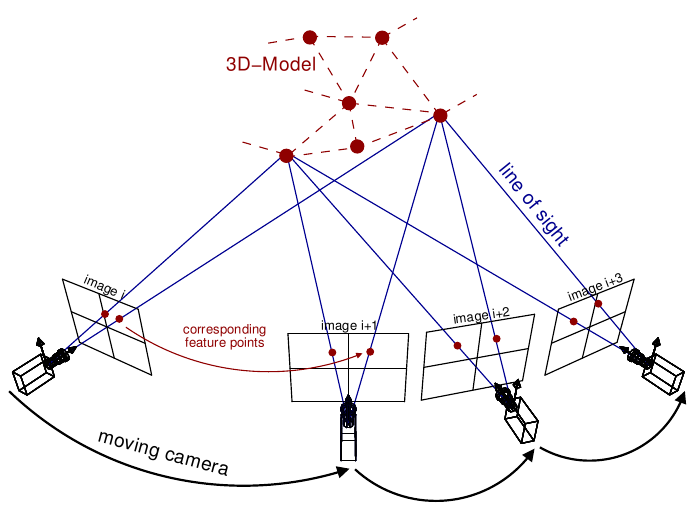
\includegraphics[width=0.4\textwidth]{assets/10_SFM.png}
\end{figure}

\section{Structured Light}
Na sledovaný objekt jsou vysílány různě velké liniové paprsky, které se zpětně snímají kamerou. Podle zakřívení povrchu je vyslaný paprsek deformován. Ze snímků deformovaných paprsků je pak možné provést triangulaci a následně zpětně rekonstruovat povrch tělesa. 

3D skener strukturovaného světla je zařízení pro měření trojrozměrného tvaru objektu užitímpromítaného svetelného vzoru a kamerového systému.V dnešní době je strukturované světlo běžně využíváno pro různé trojrozměrné profilometrické zkoumání povrchů díky jeho nízké cenně a vysoké rychlosti, proto je jedním z nejčastějších způsobů, jak velmi rychle a efektivně zjistit žádané informace o povrchu objektu. Měřící čidla na bázi strukturovaného světla (SL – structured light) jsou využívány v mnoha odvětvích, kromě strojírenství a kontroly kvality je to např. k uchování uměleckých děl, v zábavním průmyslu, medicíně nebo zabezpečení. Je to především pro jeho bezkonkurenční rozlišení, bezkontaktní zajištění rekonstrukce celého pole objektů ve vysokém rozlišení a rychlost. K výhodám se dá také jistě zařadit kompaktnost skenerů, jelikož měřící proces je realizován pouze profilometrickým systémem, který se skládá z jednotky pro zpracování a analýzu (PC), projekční jednotky (zpravidla videoprojektoru) a vizuální jednotky(CCD/CMOS kamera).Při zaznamenávání stojícího objektu je nutné, aby byl objekt stabilní. Využitím zařízení se strukturovaným světlem lze zaznamenat i geometrii pohybujícíchse těles, to se však děje na úkor snížení kvality digitalizace. Při tomto dynamickém skenování objektů se ukázalo, že základní vzory jsou nedostačující, proto začaly vznikat strukturálně složitější vzory.
\subsection{Princip}
Promítání uzkých pásů světla na trojrozměrně tvarovaný povrch vytváří linie osvětlení, které jsou zkreslené z jiného úhlu než se nachází projektor a mohou být použity pro přesnou geometrickou rekonstrukci tvaru povrchu. Používá se mnoho různých variant strukturovaného světla, ale vodorovné pruhy jsou nejčastější.


\begin{figure}[H]
    \centering
    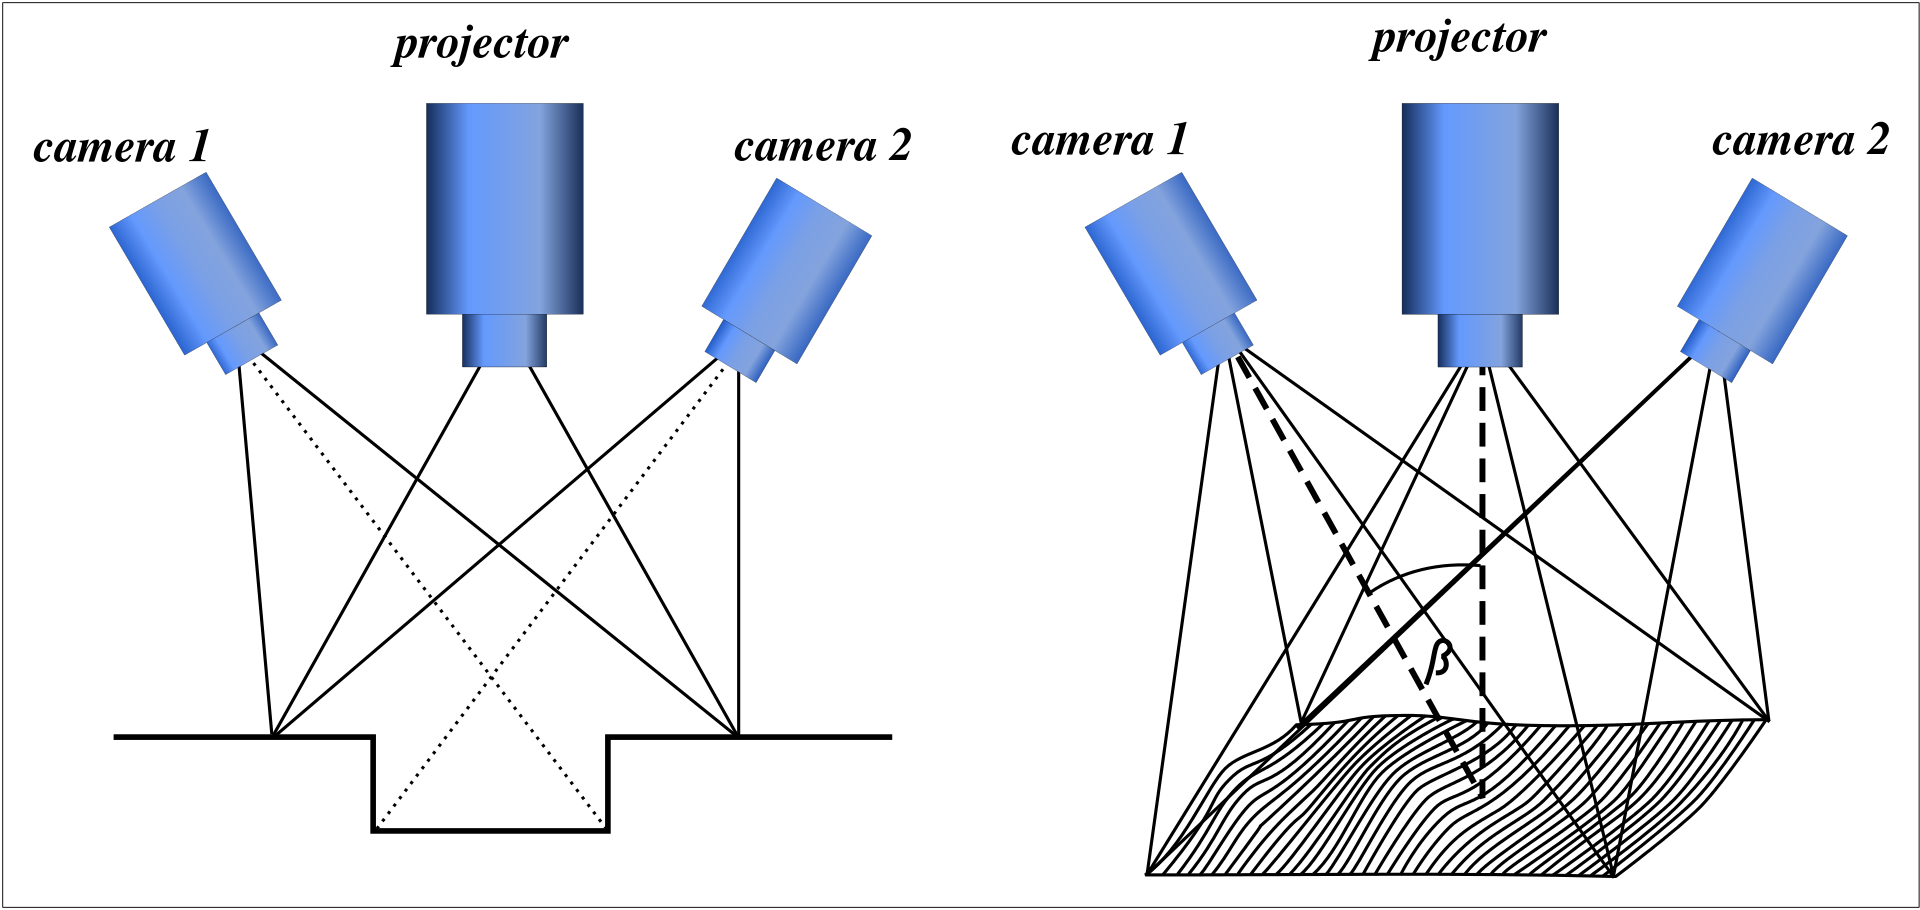
\includegraphics[width=0.4\textwidth]{assets/10_3-proj2cam.svg.png}
    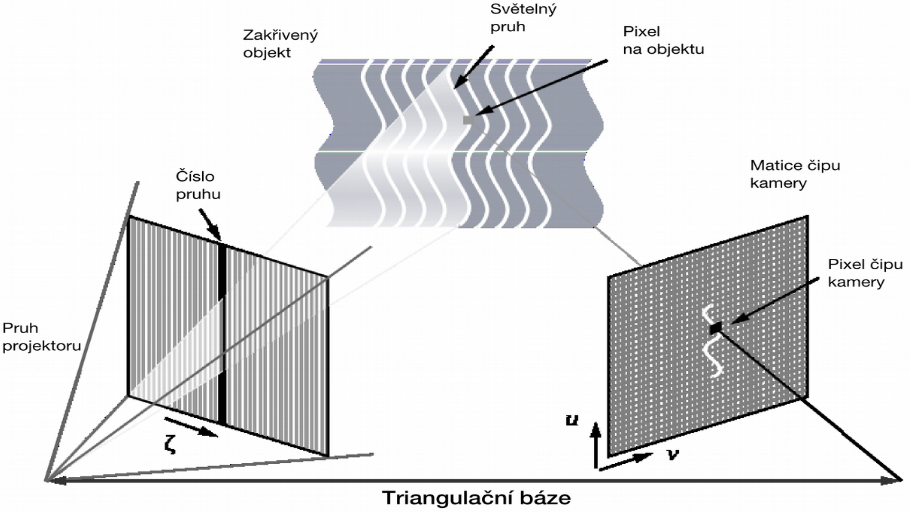
\includegraphics[width=0.4\textwidth]{assets/10_triangulaceSL.png}
\end{figure}


Modulovaný vzor je porovnán se vzorem promítaným, tj. porovnávají se odpovídající si pixely projektoru a snímacího zařízení. Výsledkem tohoto porovnání a využitím vhodného algoritmu se vytvoří body orientované v prostoru, tzv. mračna bodů.S těmito body lze dále pracovat a vytvořit souvislý povrch.